% chapters/ce1-2025-problems.tex
% GATE CE1 - Problems (BT25 format)
% Compile with XeLaTeX. Main language = English, Arabic only in heading.
% Each problem is an \item of the outer enumerate.
% Options are a nested enumerate so they are NOT numbered as problems.

\section*{\textarabic{المسائل}}    % "Problems" (only Arabic text in the document)
\setcounter{subsection}{1}         % labels become 1.1, 1.2, ...

\begin{enumerate}[label=\thesubsection.\arabic*, ref=\thesubsection.\theenumi, itemsep=0pt]

% ----------------------------------------------------------- Q3
\item At how many points will the curves $y = x^2$ and $y = -x^2 - 2x - 1$ intersect in the real $\brak{x,y}$ plane? \gate
\begin{multicols}{2}
\begin{enumerate}[label=\alph*), itemsep=0pt]
\item 0
\item 1
\item 2
\item 3
\end{enumerate}
\end{multicols}
\solution The given curves can be written in the form $\vec{x}^\top\vec{V}\vec{x} + 2\vec{u}^\top\vec{x} + f = 0$:
\begin{align}
x^2 - y = 0 &\implies \vec{V}_1 = \myvec{1 & 0\\ 0 & 0},\ \vec{u}_1 = \myvec{0\\ -\frac{1}{2}},\ f_1 = 0\\
x^2 + 2x + y + 1 = 0 &\implies \vec{V}_2 = \myvec{1 & 0\\ 0 & 0},\ \vec{u}_2 = \myvec{1\\ \frac{1}{2}},\ f_2 = 1
\end{align}
Choosing $\mu = -1$ in the pencil \eqref{eq:pencil} eliminates the second-degree terms $\brak{\vec{V}_1 - \vec{V}_2 = \vec{0}}$:
\begin{align}
2\brak{\vec{u}_1 - \vec{u}_2}^\top\vec{x} + \brak{f_1 - f_2} &= 0\\
2\myvec{-1 & -1}\vec{x} - 1 = 0 \implies \myvec{1 & 1}\vec{x} &= -\frac{1}{2}
\end{align}
All common points of the two curves lie on this line. A point on the line and its direction vector are
\begin{align}
\vec{h} = \myvec{0\\ -\frac{1}{2}},\quad \vec{m} = \myvec{1\\ -1}
\end{align}
Substituting into \eqref{eq:disc} for the first curve:
\begin{align}
\vec{m}^\top\vec{V}_1\vec{m} &= \myvec{1 & -1}\myvec{1 & 0\\ 0 & 0}\myvec{1\\ -1} = 1\\
\vec{V}_1\vec{h} + \vec{u}_1 &= \myvec{0\\ 0} + \myvec{0\\ -\frac{1}{2}} = \myvec{0\\ -\frac{1}{2}}\\
\vec{m}^\top\brak{\vec{V}_1\vec{h} + \vec{u}_1} &= \myvec{1 & -1}\myvec{0\\ -\frac{1}{2}} = \frac{1}{2}\\
g\brak{\vec{h}} &= \vec{h}^\top\vec{V}_1\vec{h} + 2\vec{u}_1^\top\vec{h} + f_1 = 0 + \frac{1}{2} + 0 = \frac{1}{2}\\
\Delta &= \brak{\frac{1}{2}}^2 - \frac{1}{2}\brak{1} = -\frac{1}{4} < 0
\end{align}
Since the discriminant is negative, $\kappa$ in \eqref{eq:kappa} is not real and the curves do not meet in the real plane.

\begin{figure}[H]
\centering
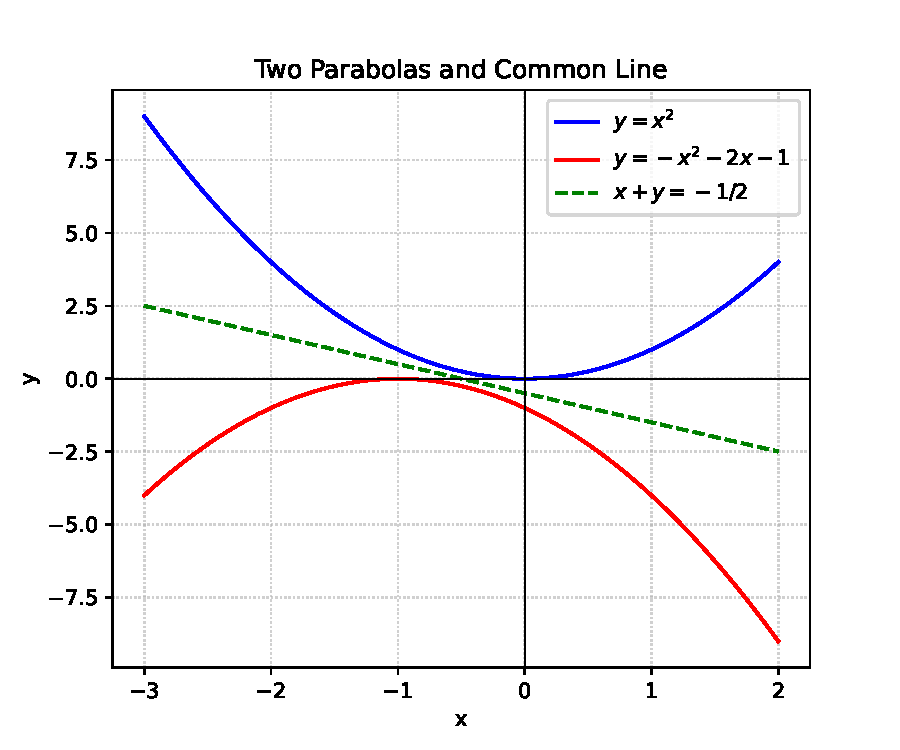
\includegraphics[width=0.85\columnwidth,keepaspectratio]{figs/q03.pdf}
\caption{The parabolas $y = x^2$ and $y = -x^2 - 2x - 1$}
\end{figure}
\begin{lstlisting}[frame=single, basicstyle=\rmfamily, escapeinside={(*@}{@*)}]
(*@\makebox[\dimexpr\linewidth-2\fboxsep-2\fboxrule\relax][c]{codes/ce1/q03.py}@*)
\end{lstlisting}
\begin{lstlisting}[frame=single, basicstyle=\rmfamily, escapeinside={(*@}{@*)}]
(*@\makebox[\dimexpr\linewidth-2\fboxsep-2\fboxrule\relax][c]{figs/q03.pdf}@*)
\end{lstlisting}

% ----------------------------------------------------------- Q7
\item In the given figure, $\overline{PQ}$ is the diameter of a circle with center $O$. Two points $R$ and $S$ are chosen on the circle such that $\angle ROS = 80^\circ$. When $\overline{PR}$ and $\overline{QS}$ are extended, they meet at $T$. The value of $\angle RTS$ is \underline{\hspace{2cm}} \gate
\begin{multicols}{2}
\begin{enumerate}[label=\alph*), itemsep=0pt]
\item $40^\circ$
\item $50^\circ$
\item $60^\circ$
\item $80^\circ$
\end{enumerate}
\end{multicols}
\solution Let $O$ be the origin and the radius be $r$. Then
\begin{align}
\vec{P} = r\vec{e}_{180^\circ} = -r\vec{e}_{0},\quad \vec{Q} = r\vec{e}_{0},\quad \vec{R} = r\vec{e}_\alpha,\quad \vec{S} = r\vec{e}_\beta
\end{align}
with $0 < \beta < \alpha < 180^\circ$ and, from \eqref{eq:cosdiff},
\begin{align}
\cos\angle ROS = \vec{e}_\alpha^\top\vec{e}_\beta = \cos\brak{\alpha-\beta} \implies \alpha - \beta = 80^\circ
\end{align}
The direction vectors of the lines $PR$ and $QS$ are
\begin{align}
\vec{R} - \vec{P} &= r\myvec{1+\cos\alpha\\ \sin\alpha} = 2r\cos\frac{\alpha}{2}\myvec{\cos\frac{\alpha}{2}\\ \sin\frac{\alpha}{2}}\\
\vec{S} - \vec{Q} &= r\myvec{\cos\beta - 1\\ \sin\beta} = 2r\sin\frac{\beta}{2}\myvec{-\sin\frac{\beta}{2}\\ \cos\frac{\beta}{2}}
\end{align}
The point $T$ lies beyond $R$ on $PR$ and beyond $S$ on $QS$. Hence $\overrightarrow{TR}$ is along $\vec{P} - \vec{R}$ and $\overrightarrow{TS}$ is along $\vec{Q} - \vec{S}$. Using \eqref{eq:angle},
\begin{align}
\cos\angle RTS &= \myvec{\cos\frac{\alpha}{2} & \sin\frac{\alpha}{2}}\myvec{-\sin\frac{\beta}{2}\\ \cos\frac{\beta}{2}}\\
&= \sin\frac{\alpha}{2}\cos\frac{\beta}{2} - \cos\frac{\alpha}{2}\sin\frac{\beta}{2} = \sin\frac{\alpha-\beta}{2}\\
&= \sin 40^\circ = \cos 50^\circ\\
\implies \angle RTS &= 50^\circ
\end{align}
For a numerical check, take $r = 1$, $\alpha = 130^\circ$, $\beta = 50^\circ$ so that $\alpha - \beta = 80^\circ$. From \eqref{eq:lineint},
\begin{align}
\myvec{\vec{R}-\vec{P} & -\brak{\vec{S}-\vec{Q}}}\myvec{\kappa_1\\ \kappa_2} = \vec{Q} - \vec{P} \implies \vec{T} = \myvec{0\\ 2.1445}
\end{align}
and \eqref{eq:angle} gives $\angle RTS = 50^\circ$.

\begin{figure}[H]
\centering
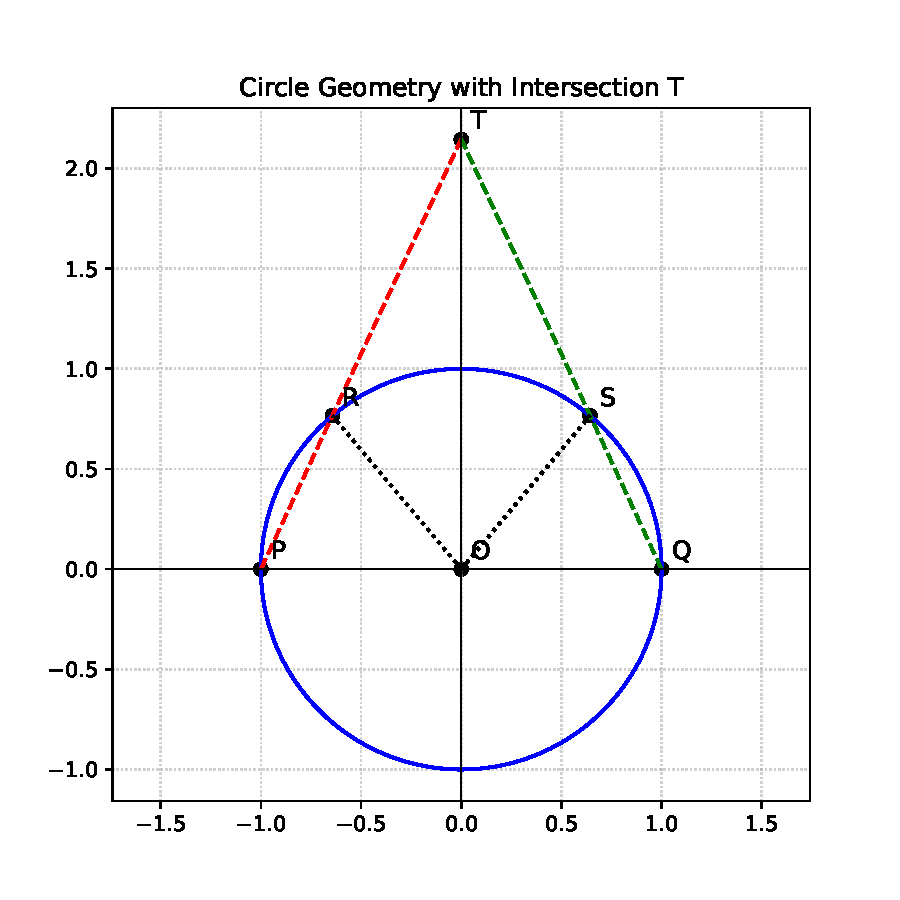
\includegraphics[width=0.85\columnwidth,keepaspectratio]{figs/q07.pdf}
\caption{Circle with diameter $PQ$, $\angle ROS = 80^\circ$ and $\angle RTS = 50^\circ$}
\end{figure}
\begin{lstlisting}[frame=single, basicstyle=\rmfamily, escapeinside={(*@}{@*)}]
(*@\makebox[\dimexpr\linewidth-2\fboxsep-2\fboxrule\relax][c]{codes/ce1/q07.py}@*)
\end{lstlisting}
\begin{lstlisting}[frame=single, basicstyle=\rmfamily, escapeinside={(*@}{@*)}]
(*@\makebox[\dimexpr\linewidth-2\fboxsep-2\fboxrule\relax][c]{figs/q07.pdf}@*)
\end{lstlisting}

% ----------------------------------------------------------- Q9
\item Consider a linear arrangement of seven bulbs, each of which can be in the ON or OFF states. The initial configuration of the bulbs is shown in the figure. In every Step, the states of the bulbs are changed based on the following rules:
Any OFF bulb with exactly one ON neighbor at the end of the previous Step is turned ON. Any ON bulb with both neighbors ON at the end of the previous Step is turned OFF. The state of any bulb not meeting the conditions above is left unchanged.
The state of bulbs at the end of Step 1 and Step 2 are also shown in the figure. The number of bulbs which are ON at the end of Step 8 is \underline{\hspace{2cm}} \gate
\begin{multicols}{2}
\begin{enumerate}[label=\alph*), itemsep=0pt]
\item 5
\item 4
\item 3
\item 0
\end{enumerate}
\end{multicols}
\solution Let $\vec{x}_k\in\cbrak{0,1}^7$ be the state vector after Step $k$ and $\vec{s}_k = \vec{A}\vec{x}_k$ from \eqref{eq:adj}, where
\begin{align}
\vec{A} = \myvec{0&1&0&0&0&0&0\\ 1&0&1&0&0&0&0\\ 0&1&0&1&0&0&0\\ 0&0&1&0&1&0&0\\ 0&0&0&1&0&1&0\\ 0&0&0&0&1&0&1\\ 0&0&0&0&0&1&0}
\end{align}
The rules give the update
\begin{align}
\vec{x}_{k+1} = \vec{x}_k + \brak{\vec{1} - \vec{x}_k}\odot\sbrak{\vec{s}_k = 1} - \vec{x}_k\odot\sbrak{\vec{s}_k = 2}
\label{eq:bulbupdate}
\end{align}
where $\odot$ is the element-wise product and $\sbrak{\cdot}$ is 1 when the condition holds. The initial configuration has only the middle bulb ON:
\begin{align}
\vec{x}_0 &= \myvec{0&0&0&1&0&0&0}^\top, & \vec{s}_0 &= \myvec{0&0&1&0&1&0&0}^\top\\
\vec{x}_1 &= \myvec{0&0&1&1&1&0&0}^\top, & \vec{s}_1 &= \myvec{0&1&1&2&1&1&0}^\top\\
\vec{x}_2 &= \myvec{0&1&1&0&1&1&0}^\top, & \vec{s}_2 &= \myvec{1&1&1&2&1&1&1}^\top\\
\vec{x}_3 &= \myvec{1&1&1&0&1&1&1}^\top, & \vec{s}_3 &= \myvec{1&2&1&2&1&2&1}^\top\\
\vec{x}_4 &= \myvec{1&0&1&0&1&0&1}^\top, & \vec{s}_4 &= \myvec{0&2&0&2&0&2&0}^\top
\end{align}
$\vec{x}_1$ and $\vec{x}_2$ agree with Step 1 and Step 2 in the figure. In $\vec{x}_4$, every OFF bulb has two ON neighbours and every ON bulb has none, so \eqref{eq:bulbupdate} gives
\begin{align}
\vec{x}_5 = \vec{x}_4 \implies \vec{x}_8 = \vec{x}_4 = \myvec{1&0&1&0&1&0&1}^\top
\end{align}
The number of ON bulbs after Step 8 is
\begin{align}
\vec{1}^\top\vec{x}_8 = 4
\end{align}

\begin{lstlisting}[frame=single, basicstyle=\rmfamily, escapeinside={(*@}{@*)}]
(*@\makebox[\dimexpr\linewidth-2\fboxsep-2\fboxrule\relax][c]{codes/ce1/q09.py}@*)
\end{lstlisting}
\begin{lstlisting}[frame=single, basicstyle=\rmfamily, escapeinside={(*@}{@*)}]
(*@\makebox[\dimexpr\linewidth-2\fboxsep-2\fboxrule\relax][c]{figs/q09.pdf}@*)
\end{lstlisting}

% ----------------------------------------------------------- Q10
\item $P$ and $Q$ are two positive integers such that $P^2 = Q^2 + 13$. The product of the numbers $P$ and $Q$ is \underline{\hspace{2cm}} \gate
\begin{multicols}{2}
\begin{enumerate}[label=\alph*), itemsep=0pt]
\item 13
\item 26
\item 39
\item 42
\end{enumerate}
\end{multicols}
\solution The given equation can be written as
\begin{align}
P^2 - Q^2 = \brak{P-Q}\brak{P+Q} = 13
\end{align}
Since 13 is prime and $0 < P - Q < P + Q$,
\begin{align}
P - Q = 1,\quad P + Q = 13
\end{align}
Expressing in the matrix form \eqref{eq:axb}:
\begin{align}
\myvec{1 & -1\\ 1 & 1}\myvec{P\\ Q} = \myvec{1\\ 13}
\end{align}
Applying $R_2 \to R_2 - R_1$ on the augmented matrix:
\begin{align}
\myvec{1 & -1 & 1\\ 1 & 1 & 13} \xrightarrow{R_2\to R_2 - R_1} \myvec{1 & -1 & 1\\ 0 & 2 & 12} \implies Q = 6,\ P = 7
\end{align}
Therefore,
\begin{align}
PQ = 7\times 6 = 42
\end{align}

\begin{lstlisting}[frame=single, basicstyle=\rmfamily, escapeinside={(*@}{@*)}]
(*@\makebox[\dimexpr\linewidth-2\fboxsep-2\fboxrule\relax][c]{codes/ce1/q10.py}@*)
\end{lstlisting}

% ----------------------------------------------------------- Q11 (1.1.15)
\item Matrix $\vec{P}$ is given as
\begin{align}
\vec{P} = \myvec{1 & 0 & 1\\ 0 & 1 & 0\\ 1 & 0 & 1}
\end{align}
The TRUE option is \gate
\begin{multicols}{2}
\begin{enumerate}[label=\alph*), itemsep=0pt]
\item Trace of $\vec{P}$ is equal to the sum of the Eigen values of $\vec{P}$.
\item $\vec{P}^\top\vec{P}$ is an identity matrix.
\item $\vec{P}$ is a skew-symmetric matrix.
\item Absolute magnitude of each Eigen value is 1.
\end{enumerate}
\end{multicols}
\solution From \eqref{eq:charpoly}, expanding along the second row,
\begin{align}
\abs{\lambda\vec{I} - \vec{P}} &= \mydet{\lambda-1 & 0 & -1\\ 0 & \lambda-1 & 0\\ -1 & 0 & \lambda-1}\\
&= \brak{\lambda-1}\sbrak{\brak{\lambda-1}^2 - 1}\\
&= \lambda\brak{\lambda-1}\brak{\lambda-2} = 0\\
\implies \lambda_1 &= 0,\ \lambda_2 = 1,\ \lambda_3 = 2
\end{align}
From \eqref{eq:trace}:
\begin{align}
\text{tr}\brak{\vec{P}} = 1+1+1 = 3 = \lambda_1 + \lambda_2 + \lambda_3
\end{align}
so option (A) is true. The remaining options are false since
\begin{align}
\vec{P}^\top\vec{P} &= \myvec{2 & 0 & 2\\ 0 & 1 & 0\\ 2 & 0 & 2} \neq \vec{I}\\
\vec{P}^\top &= \vec{P} \neq -\vec{P}\\
\abs{\lambda_1} &= 0 \neq 1
\end{align}
\begin{lstlisting}[frame=single, basicstyle=\rmfamily, escapeinside={(*@}{@*)}]
(*@\makebox[\dimexpr\linewidth-2\fboxsep-2\fboxrule\relax][c]{codes/ce1/q11.py}@*)
\end{lstlisting}

% ----------------------------------------------------------- Q12
\item Given:
\begin{align}
\myvec{1 & 1 & 1\\ 1 & 0 & 2}\myvec{x_1\\ x_2\\ x_3} = \myvec{0\\ 0}
\end{align}
The above system of equations represents a \gate
\begin{multicols}{2}
\begin{enumerate}[label=\alph*), itemsep=0pt]
\item plane
\item line
\item volume
\item point
\end{enumerate}
\end{multicols}
\solution The augmented matrix is reduced as
\begin{align}
\myvec{1 & 1 & 1 & 0\\ 1 & 0 & 2 & 0} \xrightarrow{R_2\to R_2 - R_1} \myvec{1 & 1 & 1 & 0\\ 0 & -1 & 1 & 0}
\end{align}
Thus,
\begin{align}
\text{rank}\brak{\vec{A}} = \text{rank}\brak{\sbrak{\vec{A}\mid\vec{b}}} = 2 < n = 3
\end{align}
From \eqref{eq:rc}, the system is consistent with $n - r = 1$ free variable. From \eqref{eq:cross}, the solution is
\begin{align}
\vec{x} = \kappa\brak{\myvec{1\\ 1\\ 1}\times\myvec{1\\ 0\\ 2}} = \kappa\myvec{2\\ -1\\ -1},\quad \kappa\in\mathbb{R}
\end{align}
which is a line through the origin (the intersection of two planes).

\begin{figure}[H]
\centering
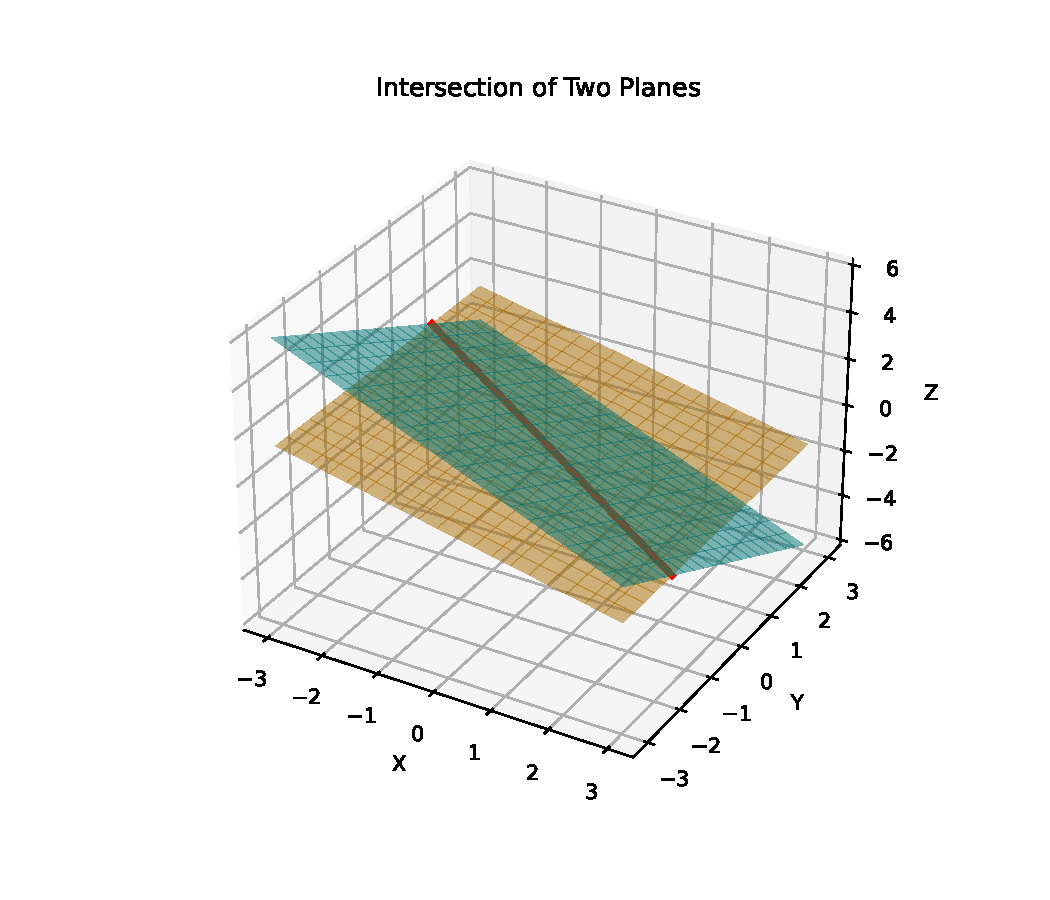
\includegraphics[width=0.85\columnwidth,keepaspectratio]{figs/q12.pdf}
\caption{The two planes and their line of intersection}
\end{figure}
\begin{lstlisting}[frame=single, basicstyle=\rmfamily, escapeinside={(*@}{@*)}]
(*@\makebox[\dimexpr\linewidth-2\fboxsep-2\fboxrule\relax][c]{codes/ce1/q12.py}@*)
\end{lstlisting}
\begin{lstlisting}[frame=single, basicstyle=\rmfamily, escapeinside={(*@}{@*)}]
(*@\makebox[\dimexpr\linewidth-2\fboxsep-2\fboxrule\relax][c]{figs/q12.pdf}@*)
\end{lstlisting}

% ----------------------------------------------------------- Q26
\item Bag I contains 4 white and 6 black balls. Bag II contains 4 white and 3 black balls. One ball is drawn at random from any one of the two bags and it is found to be a black ball. The probability that the black ball was drawn from Bag I is \underline{\hspace{2cm}} (rounded off to two decimal places). \gate

\solution Let $B_1$, $B_2$ denote choosing Bag I, Bag II and $E$ the event of drawing a black ball. The prior and likelihood vectors are
\begin{align}
\vec{\pi} = \myvec{\frac{1}{2}\\ \frac{1}{2}},\quad \vec{l} = \myvec{\frac{6}{10}\\ \frac{3}{7}}
\end{align}
From \eqref{eq:total},
\begin{align}
\pr{E} = \vec{\pi}^\top\vec{l} = \frac{1}{2}\brak{\frac{3}{5} + \frac{3}{7}} = \frac{18}{35}
\end{align}
From \eqref{eq:bayes},
\begin{align}
\pr{B_1\mid E} = \frac{\frac{1}{2}\times\frac{3}{5}}{\frac{18}{35}} = \frac{3}{10}\times\frac{35}{18} = \frac{7}{12} \approx 0.58
\end{align}
\begin{lstlisting}[frame=single, basicstyle=\rmfamily, escapeinside={(*@}{@*)}]
(*@\makebox[\dimexpr\linewidth-2\fboxsep-2\fboxrule\relax][c]{codes/ce1/q26.py}@*)
\end{lstlisting}

% ----------------------------------------------------------- Q27
\item A matrix is given as:
\begin{align}
\myvec{9 & 15\\ 15 & 50}
\end{align}
By performing Cholesky decomposition, $\abs{l_{22}}$ of the lower triangular matrix is \underline{\hspace{2cm}} (in integer). \gate

\solution Comparing with \eqref{eq:chol2},
\begin{align}
l_{11}^2 &= 9 \implies l_{11} = 3\\
l_{11}l_{21} &= 15 \implies l_{21} = 5\\
l_{21}^2 + l_{22}^2 &= 50 \implies l_{22}^2 = 25 \implies \abs{l_{22}} = 5
\end{align}
Thus,
\begin{align}
\vec{L} = \myvec{3 & 0\\ 5 & 5},\quad \vec{L}\vec{L}^\top = \myvec{9 & 15\\ 15 & 50}
\end{align}
\begin{lstlisting}[frame=single, basicstyle=\rmfamily, escapeinside={(*@}{@*)}]
(*@\makebox[\dimexpr\linewidth-2\fboxsep-2\fboxrule\relax][c]{codes/ce1/q27.py}@*)
\end{lstlisting}

% ----------------------------------------------------------- Q28
\item It is given that $x$ and $y$ are integers in the following equation:
\begin{align}
\brak{x + y - 7}^2 + \brak{y + 3x - 13}^2 = 0
\end{align}
The value of $\brak{x^3 + y^3}$ is \underline{\hspace{2cm}} (in integer). \gate

\solution Let
\begin{align}
\vec{A} = \myvec{1 & 1\\ 3 & 1},\quad \vec{b} = \myvec{7\\ 13},\quad \vec{x} = \myvec{x\\ y}
\end{align}
The given equation is
\begin{align}
\norm{\vec{A}\vec{x} - \vec{b}}^2 = 0
\end{align}
From \eqref{eq:zeronorm},
\begin{align}
\vec{A}\vec{x} = \vec{b}
\end{align}
Reducing the augmented matrix:
\begin{align}
\myvec{1 & 1 & 7\\ 3 & 1 & 13} \xrightarrow{R_2\to R_2 - 3R_1} \myvec{1 & 1 & 7\\ 0 & -2 & -8} \implies y = 4,\ x = 3
\end{align}
Therefore,
\begin{align}
x^3 + y^3 = 27 + 64 = 91
\end{align}
\begin{lstlisting}[frame=single, basicstyle=\rmfamily, escapeinside={(*@}{@*)}]
(*@\makebox[\dimexpr\linewidth-2\fboxsep-2\fboxrule\relax][c]{codes/ce1/q28.py}@*)
\end{lstlisting}

% ----------------------------------------------------------- Q33
\item The travel times of three vehicles on a 2 km stretch of road are 4, 5, and 8 minutes. Assuming the speed of each vehicle to be constant in this stretch, the Space Mean Speed (in km/h) of the vehicles is \underline{\hspace{2cm}} (rounded off to two decimal places). \gate

\solution The travel time vector (in hours) is
\begin{align}
\vec{t} = \frac{1}{60}\myvec{4\\ 5\\ 8},\quad \vec{1}^\top\vec{t} = \frac{17}{60}\text{ h}
\end{align}
From \eqref{eq:sms} with $n = 3$ and $d = 2$ km,
\begin{align}
v_s = \frac{nd}{\vec{1}^\top\vec{t}} = \frac{3\times 2}{\frac{17}{60}} = \frac{360}{17} \approx 21.18\text{ km/h}
\end{align}
Equivalently, the spot speeds are $\myvec{30 & 24 & 15}$ km/h and their harmonic mean is
\begin{align}
v_s = \frac{3}{\frac{1}{30} + \frac{1}{24} + \frac{1}{15}} = 21.18\text{ km/h}
\end{align}
\begin{lstlisting}[frame=single, basicstyle=\rmfamily, escapeinside={(*@}{@*)}]
(*@\makebox[\dimexpr\linewidth-2\fboxsep-2\fboxrule\relax][c]{codes/ce1/q33.py}@*)
\end{lstlisting}

% ----------------------------------------------------------- Q35
\item The height of the plane of collimation of a levelling instrument is 100.000 m from a datum. The levelling instrument measures a Back Sight of 1.500 m on a vertically held staff at a ground point $P$. The reduced level (in m) of the ground point $P$ with respect to the datum is \underline{\hspace{2cm}} (rounded off to three decimal places). \gate

\solution From \eqref{eq:rl},
\begin{align}
\text{RL}_P = \text{HI} - h = 100.000 - 1.500 = 98.500\text{ m}
\end{align}
\begin{lstlisting}[frame=single, basicstyle=\rmfamily, escapeinside={(*@}{@*)}]
(*@\makebox[\dimexpr\linewidth-2\fboxsep-2\fboxrule\relax][c]{codes/ce1/q35.py}@*)
\end{lstlisting}

% ----------------------------------------------------------- Q36
\item Let $f\brak{x}$ be a continuous function defined in $\sbrak{0,2}\to\mathbb{R}$ and satisfying the equation
\begin{align}
\int_0^2 f\brak{x}\sbrak{x - f\brak{x}}dx = \frac{2}{3}
\end{align}
The value of $f\brak{1}$ is \gate
\begin{multicols}{2}
\begin{enumerate}[label=\alph*), itemsep=0pt]
\item 1
\item 2
\item $\frac{1}{2}$
\item 0
\end{enumerate}
\end{multicols}
\solution Using \eqref{eq:cts} with $a = x$ and $b = f\brak{x}$:
\begin{align}
f\brak{x}\sbrak{x - f\brak{x}} = \frac{x^2}{4} - \brak{f\brak{x} - \frac{x}{2}}^2
\end{align}
Integrating over $\sbrak{0,2}$:
\begin{align}
\int_0^2 f\brak{x}\sbrak{x - f\brak{x}}dx &= \int_0^2\frac{x^2}{4}dx - \int_0^2\brak{f\brak{x} - \frac{x}{2}}^2dx\\
&= \frac{2}{3} - \int_0^2\brak{f\brak{x} - \frac{x}{2}}^2dx
\end{align}
Equating with the given value,
\begin{align}
\int_0^2\brak{f\brak{x} - \frac{x}{2}}^2dx = 0
\end{align}
Since the integrand is continuous and non-negative,
\begin{align}
f\brak{x} = \frac{x}{2} \implies f\brak{1} = \frac{1}{2}
\end{align}

\begin{figure}[H]
\centering
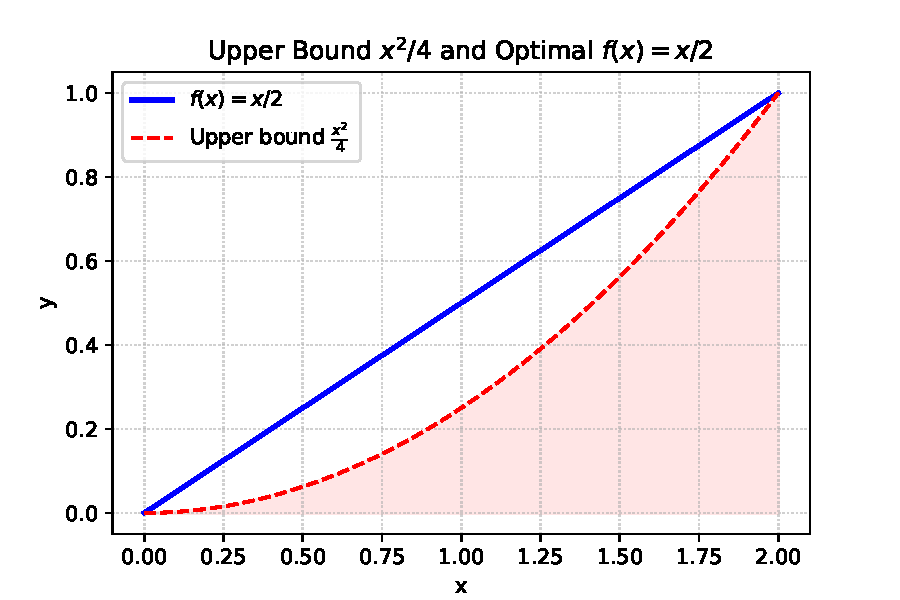
\includegraphics[width=0.85\columnwidth,keepaspectratio]{figs/q36.pdf}
\caption{The integrand attains its upper bound $\frac{x^2}{4}$ only for $f\brak{x} = \frac{x}{2}$}
\end{figure}
\begin{lstlisting}[frame=single, basicstyle=\rmfamily, escapeinside={(*@}{@*)}]
(*@\makebox[\dimexpr\linewidth-2\fboxsep-2\fboxrule\relax][c]{codes/ce1/q36.py}@*)
\end{lstlisting}
\begin{lstlisting}[frame=single, basicstyle=\rmfamily, escapeinside={(*@}{@*)}]
(*@\makebox[\dimexpr\linewidth-2\fboxsep-2\fboxrule\relax][c]{figs/q36.pdf}@*)
\end{lstlisting}

% ----------------------------------------------------------- Q37
\item An ordinary differential equation is given below.
\begin{align}
x^2\frac{d^2y}{dx^2} = 6y
\end{align}
Considering $a$ and $b$ as arbitrary constants, the general solution of the equation is \gate
\begin{multicols}{2}
\begin{enumerate}[label=\alph*), itemsep=0pt]
\item $y\brak{x} = ax^3 + \frac{b}{x^2}$
\item $y\brak{x} = ax^2 + \frac{b}{x^3}$
\item $y\brak{x} = ax^2 + b\ln x$
\item $y\brak{x} = ax^3 + b\ln x$
\end{enumerate}
\end{multicols}
\solution Let $x = e^t$ $\brak{x > 0}$. Then
\begin{align}
x\frac{dy}{dx} = \frac{dy}{dt},\quad x^2\frac{d^2y}{dx^2} = \frac{d^2y}{dt^2} - \frac{dy}{dt}
\end{align}
and the equation becomes
\begin{align}
y'' - y' - 6y = 0
\label{eq:q37t}
\end{align}
Taking the Laplace transform using \eqref{eq:lap1} and \eqref{eq:lap2}:
\begin{align}
s^2Y\brak{s} - sy\brak{0} - y'\brak{0} - \sbrak{sY\brak{s} - y\brak{0}} - 6Y\brak{s} &= 0\\
Y\brak{s} = \frac{\brak{s-1}y\brak{0} + y'\brak{0}}{s^2 - s - 6} &= \frac{\brak{s-1}y\brak{0} + y'\brak{0}}{\brak{s-3}\brak{s+2}}
\end{align}
Decomposing into partial fractions and using \eqref{eq:lapexp},
\begin{align}
Y\brak{s} = \frac{a}{s-3} + \frac{b}{s+2} \implies y\brak{t} = ae^{3t} + be^{-2t}
\end{align}
Equivalently, from \eqref{eq:ss}, the exponents are the eigenvalues of
\begin{align}
\vec{A} = \myvec{0 & 1\\ 6 & 1},\quad \abs{\lambda\vec{I} - \vec{A}} = \lambda^2 - \lambda - 6 = 0 \implies \lambda = 3, -2
\end{align}
Substituting $e^t = x$:
\begin{align}
y\brak{x} = ax^3 + \frac{b}{x^2}
\end{align}

\begin{lstlisting}[frame=single, basicstyle=\rmfamily, escapeinside={(*@}{@*)}]
(*@\makebox[\dimexpr\linewidth-2\fboxsep-2\fboxrule\relax][c]{codes/ce1/q37.py}@*)
\end{lstlisting}

% ----------------------------------------------------------- Q38
\item A plane truss consists of two linearly elastic, homogeneous, identical members, namely $PQ$ and $QR$. Both members have length $\brak{L}$, cross-sectional area $\brak{A}$, and modulus of elasticity $\brak{E}$. The members are inclined at $45^\circ$ as shown in the figure. The truss has hinge supports at $P$ and $R$. The translational degrees-of-freedom ($u$ and $v$) are shown at joint $Q$.

After application of the boundary conditions, the stiffness matrix of the truss becomes: \gate
\begin{multicols}{2}
\begin{enumerate}[label=\alph*), itemsep=0pt]
\item $\frac{AE}{L}\myvec{1 & 1\\ 1 & 1}$
\item $\frac{AE}{L}\myvec{1 & 0.5\\ 0.5 & 1}$
\item $\frac{AE}{L}\myvec{1 & 0\\ 0 & 1}$
\item $\frac{AE}{L}\myvec{1 & -1\\ -1 & 1}$
\end{enumerate}
\end{multicols}
\solution The unit direction vectors of the members are
\begin{align}
\vec{m}_{PQ} = \frac{1}{\sqrt{2}}\myvec{1\\ 1},\quad \vec{m}_{QR} = \frac{1}{\sqrt{2}}\myvec{1\\ -1}
\end{align}
From \eqref{eq:kbar},
\begin{align}
\vec{k}_{PQ} &= \frac{AE}{L}\vec{m}_{PQ}\vec{m}_{PQ}^\top = \frac{AE}{L}\myvec{0.5 & 0.5\\ 0.5 & 0.5}\\
\vec{k}_{QR} &= \frac{AE}{L}\vec{m}_{QR}\vec{m}_{QR}^\top = \frac{AE}{L}\myvec{0.5 & -0.5\\ -0.5 & 0.5}
\end{align}
After deleting the restrained degrees of freedom at $P$ and $R$, only the $\brak{u,v}$ block at $Q$ receives contributions from both members:
\begin{align}
\vec{K} = \vec{k}_{PQ} + \vec{k}_{QR} = \frac{AE}{L}\myvec{1 & 0\\ 0 & 1}
\end{align}

\begin{figure}[H]
\centering
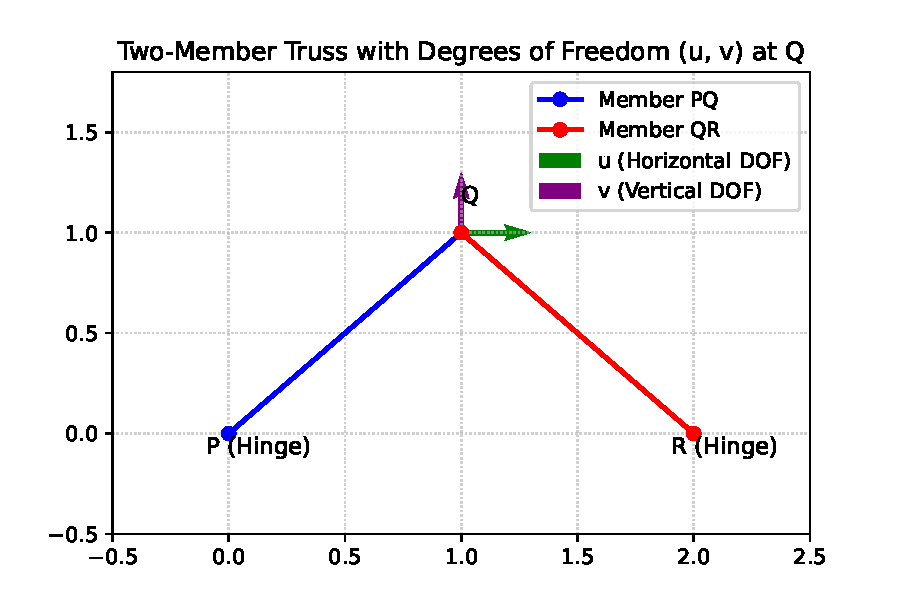
\includegraphics[width=0.85\columnwidth,keepaspectratio]{figs/q38.pdf}
\caption{Two-member truss with degrees of freedom $u$, $v$ at $Q$}
\end{figure}
\begin{lstlisting}[frame=single, basicstyle=\rmfamily, escapeinside={(*@}{@*)}]
(*@\makebox[\dimexpr\linewidth-2\fboxsep-2\fboxrule\relax][c]{codes/ce1/q38.py}@*)
\end{lstlisting}
\begin{lstlisting}[frame=single, basicstyle=\rmfamily, escapeinside={(*@}{@*)}]
(*@\makebox[\dimexpr\linewidth-2\fboxsep-2\fboxrule\relax][c]{figs/q38.pdf}@*)
\end{lstlisting}

% ----------------------------------------------------------- Q39
\item The plane frame has a hinge and a roller support, and is loaded as shown in the figure. Both the columns have same height.

What is the absolute value of the maximum bending moment (in kN-m) in the frame? \gate
\begin{multicols}{2}
\begin{enumerate}[label=\alph*), itemsep=0pt]
\item 165
\item 150
\item 240
\item 195
\end{enumerate}
\end{multicols}
\solution From the figure, the frame has a hinge at $A$, a roller at $B$, columns of height 3 m and a beam $CD$ of span 4 m. A horizontal load of 50 kN acts at $C$ and a vertical load of 90 kN acts at the mid-point $E$ of $CD$:
\begin{align}
\vec{A} = \myvec{0\\ 0},\ \vec{C} = \myvec{0\\ 3},\ \vec{E} = \myvec{2\\ 3},\ \vec{D} = \myvec{4\\ 3},\ \vec{B} = \myvec{4\\ 0},\quad \vec{F}_C = \myvec{50\\ 0},\ \vec{F}_E = \myvec{0\\ -90}
\end{align}
The reactions are $\vec{R}_A = \myvec{H_A & V_A}^\top$ and $\vec{R}_B = \myvec{0 & V_B}^\top$. From \eqref{eq:equil} with moments about $\vec{A}$,
\begin{align}
\brak{\vec{C}-\vec{A}}\times\vec{F}_C &= 0\times 0 - 3\times 50 = -150\\
\brak{\vec{E}-\vec{A}}\times\vec{F}_E &= 2\times\brak{-90} - 3\times 0 = -180\\
\brak{\vec{B}-\vec{A}}\times\vec{R}_B &= 4V_B
\end{align}
In matrix form:
\begin{align}
\myvec{1 & 0 & 0\\ 0 & 1 & 1\\ 0 & 0 & 4}\myvec{H_A\\ V_A\\ V_B} = \myvec{-50\\ 90\\ 330} \implies \myvec{H_A\\ V_A\\ V_B} = \myvec{-50\\ 7.5\\ 82.5}\text{ kN}
\end{align}
Using \eqref{eq:bm}, the bending moment in column $AC$ at height $y$ (forces below the section) is
\begin{align}
\abs{M} = \abs{\brak{\vec{A} - \myvec{0\\ y}}\times\vec{R}_A} = 50y \implies \abs{M_C} = 150\text{ kN m}
\end{align}
and in the beam at $E$ (forces to the right of the section) is
\begin{align}
\abs{M_E} = \abs{\brak{\vec{B} - \vec{E}}\times\vec{R}_B} = \abs{2\times 82.5 - \brak{-3}\times 0} = 165\text{ kN m}
\end{align}
In column $BD$, the roller reaction is vertical and along the column, so $M = 0$.
The maximum bending moment is 165 kN m under the 90 kN load.

\begin{figure}[H]
\centering
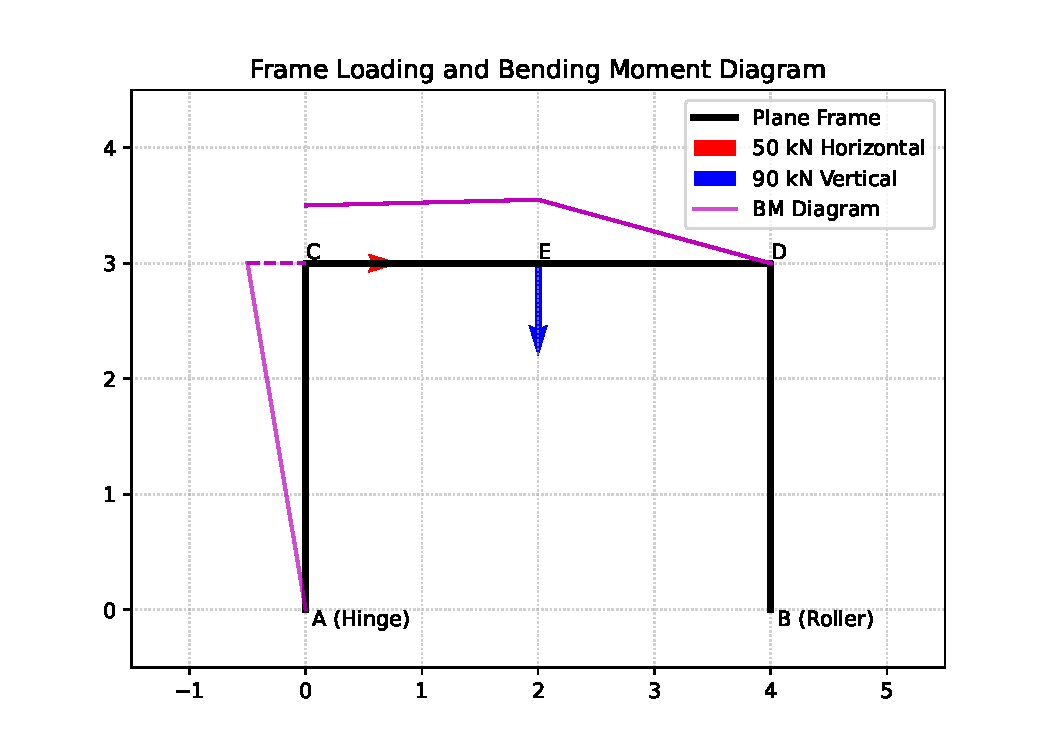
\includegraphics[width=0.85\columnwidth,keepaspectratio]{figs/q39.pdf}
\caption{Frame loading and bending moment diagram}
\end{figure}
\begin{lstlisting}[frame=single, basicstyle=\rmfamily, escapeinside={(*@}{@*)}]
(*@\makebox[\dimexpr\linewidth-2\fboxsep-2\fboxrule\relax][c]{codes/ce1/q39.py}@*)
\end{lstlisting}
\begin{lstlisting}[frame=single, basicstyle=\rmfamily, escapeinside={(*@}{@*)}]
(*@\makebox[\dimexpr\linewidth-2\fboxsep-2\fboxrule\relax][c]{figs/q39.pdf}@*)
\end{lstlisting}

% ----------------------------------------------------------- Q48
\item Starting with the first approximation as $x = 0.5$, the second approximation for the root of the following function by the Newton-Raphson method is \underline{\hspace{2cm}} (rounded off to two decimal places).
\begin{align}
f\brak{x} = e^{-x} - x
\end{align}
\gate

\solution The function and its derivative are
\begin{align}
f\brak{x} &= e^{-x} - x\\
f'\brak{x} &= -e^{-x} - 1
\end{align}
Substituting into \eqref{eq:nr}:
\begin{align}
x_{n+1} &= x_n + \frac{e^{-x_n} - x_n}{e^{-x_n} + 1}\\
&= \frac{1 + x_n}{1 + e^{x_n}}
\end{align}
With the first approximation $x_0 = 0.5$, the second approximation is
\begin{align}
x_1 = \frac{1.5}{1 + e^{0.5}} = \frac{1.5}{2.64872} = 0.56631 \approx 0.57
\end{align}
Subsequent iterations converge to $x_2 = x_3 = 0.567143$.

\begin{figure}[H]
\centering
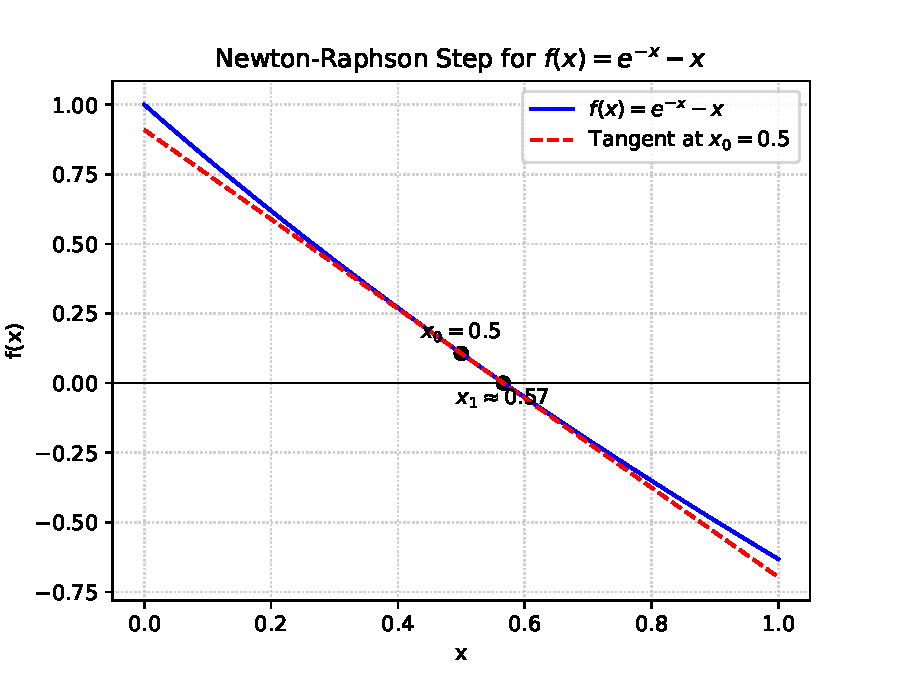
\includegraphics[width=0.85\columnwidth,keepaspectratio]{figs/q48.pdf}
\caption{One Newton-Raphson step for $f\brak{x} = e^{-x} - x$ from $x_0 = 0.5$}
\end{figure}
\begin{lstlisting}[frame=single, basicstyle=\rmfamily, escapeinside={(*@}{@*)}]
(*@\makebox[\dimexpr\linewidth-2\fboxsep-2\fboxrule\relax][c]{codes/ce1/q48.py}@*)
\end{lstlisting}
\begin{lstlisting}[frame=single, basicstyle=\rmfamily, escapeinside={(*@}{@*)}]
(*@\makebox[\dimexpr\linewidth-2\fboxsep-2\fboxrule\relax][c]{figs/q48.pdf}@*)
\end{lstlisting}

% ----------------------------------------------------------- Q49
\item Values of $y$ for different values of $x$ are tabulated below.
\begin{center}
\begin{tabular}{|c|c|c|c|}
\hline
$x$ & $-2$ & 1 & 2\\ \hline
$y$ & 28 & 4 & 16\\ \hline
\end{tabular}
\end{center}
If a second-degree interpolating polynomial $P_2\brak{x}$ is used to represent $y$, the value of $P_2\brak{0}$ is \underline{\hspace{2cm}} (rounded off to the nearest integer). \gate

\solution Let $\vec{c} = \myvec{c_0 & c_1 & c_2}^\top$ and $\vec{y} = \myvec{28 & 4 & 16}^\top$. From \eqref{eq:vander},
\begin{align}
\myvec{1 & -2 & 4\\ 1 & 1 & 1\\ 1 & 2 & 4}\vec{c} = \vec{y}
\end{align}
Reducing the augmented matrix:
\begin{align}
\myvec{1 & -2 & 4 & 28\\ 1 & 1 & 1 & 4\\ 1 & 2 & 4 & 16}
&\xrightarrow[R_3\to R_3 - R_1]{R_2\to R_2 - R_1}
\myvec{1 & -2 & 4 & 28\\ 0 & 3 & -3 & -24\\ 0 & 4 & 0 & -12}\\
&\implies c_1 = -3,\ c_2 = 5,\ c_0 = 2
\end{align}
Thus,
\begin{align}
\vec{c} = \myvec{2\\ -3\\ 5} \implies P_2\brak{x} = 5x^2 - 3x + 2
\end{align}
and
\begin{align}
P_2\brak{0} = \myvec{1 & 0 & 0}\vec{c} = 2
\end{align}

\begin{figure}[H]
\centering
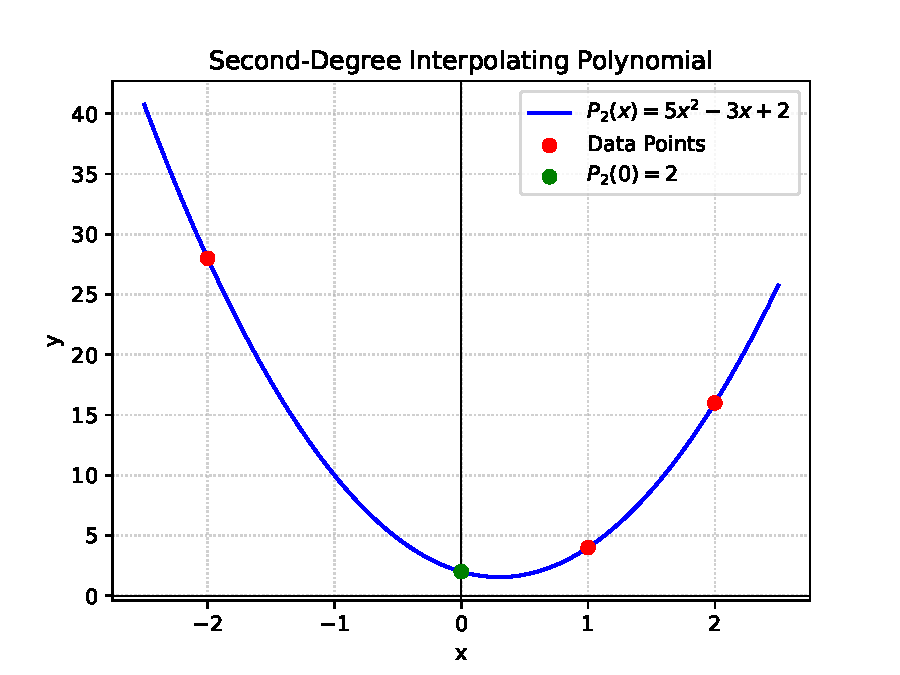
\includegraphics[width=0.85\columnwidth,keepaspectratio]{figs/q49.pdf}
\caption{Interpolating polynomial through the given points}
\end{figure}
\begin{lstlisting}[frame=single, basicstyle=\rmfamily, escapeinside={(*@}{@*)}]
(*@\makebox[\dimexpr\linewidth-2\fboxsep-2\fboxrule\relax][c]{codes/ce1/q49.py}@*)
\end{lstlisting}
\begin{lstlisting}[frame=single, basicstyle=\rmfamily, escapeinside={(*@}{@*)}]
(*@\makebox[\dimexpr\linewidth-2\fboxsep-2\fboxrule\relax][c]{figs/q49.pdf}@*)
\end{lstlisting}

% ----------------------------------------------------------- Q50
\item Two identical blocks $A$ and $B$ are connected by a rigid rod. The blocks rest against vertical and horizontal planes, as shown in the figure. The coefficient of static friction at the vertical and horizontal planes is the same. If the sliding impends when $\theta = 45^\circ$, the value of the coefficient of static friction is \underline{\hspace{2cm}} (rounded off to two decimal places). \gate

\solution Let each block have weight $W$ and let the rod make angle $\theta$ with the horizontal, with $c = \cos\theta$, $s = \sin\theta$. The rod is a two-force member carrying compression $C$ along
\begin{align}
\vec{e} = \frac{\vec{A} - \vec{B}}{\norm{\vec{A} - \vec{B}}} = \myvec{-c\\ s}
\end{align}
When sliding impends, $A$ moves down and $B$ moves away from the wall, so the friction forces are $\mu N_A$ (upward on $A$) and $\mu N_B$ (towards the wall on $B$). From \eqref{eq:equil}:
\begin{align}
\text{Block }A:&\quad \myvec{N_A\\ \mu N_A} + \myvec{0\\ -W} + C\myvec{-c\\ s} = \vec{0}\\
\text{Block }B:&\quad \myvec{-\mu N_B\\ N_B} + \myvec{0\\ -W} - C\myvec{-c\\ s} = \vec{0}
\end{align}
This gives four equations in three unknowns $\myvec{N_A & N_B & C}^\top$:
\begin{align}
\myvec{1 & 0 & -c\\ \mu & 0 & s\\ 0 & -\mu & c\\ 0 & 1 & -s}\myvec{N_A\\ N_B\\ C} = \myvec{0\\ W\\ 0\\ W}
\end{align}
From \eqref{eq:augdet}, the system is consistent only if
\begin{align}
\mydet{1 & 0 & -c & 0\\ \mu & 0 & s & W\\ 0 & -\mu & c & 0\\ 0 & 1 & -s & W} = 0
\end{align}
Expanding along the second column,
\begin{align}
\mu\mydet{1 & -c & 0\\ \mu & s & W\\ 0 & -s & W} + \mydet{1 & -c & 0\\ \mu & s & W\\ 0 & c & 0} &= 0\\
\mu W\brak{2s + \mu c} - Wc &= 0\\
\implies \tan\theta &= \frac{1 - \mu^2}{2\mu}
\end{align}
For $\theta = 45^\circ$:
\begin{align}
\mu^2 + 2\mu - 1 = 0 \implies \mu = -1 + \sqrt{2} = 0.414
\end{align}
taking the positive root.

\begin{figure}[H]
\centering
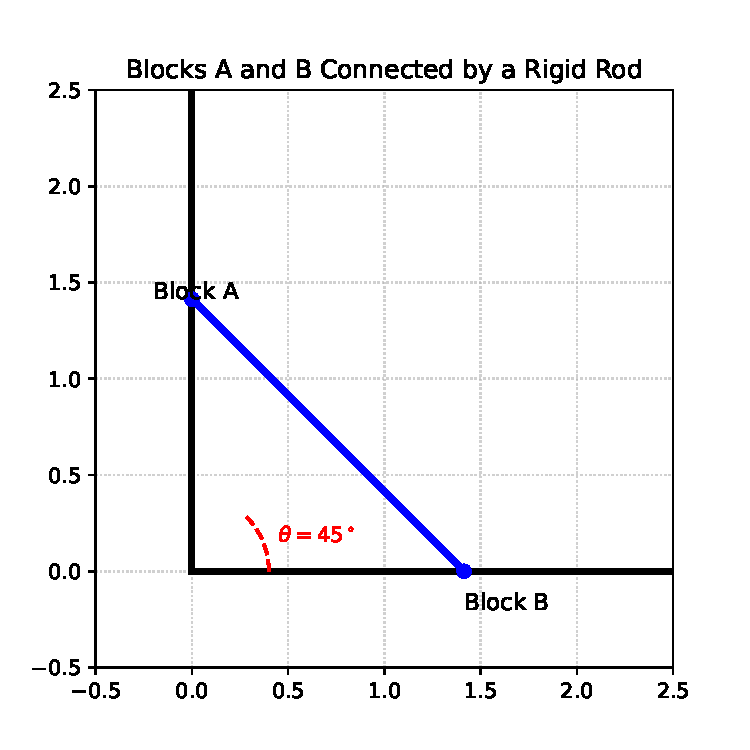
\includegraphics[width=0.85\columnwidth,keepaspectratio]{figs/q50.pdf}
\caption{Blocks $A$ and $B$ connected by a rigid rod at $\theta = 45^\circ$}
\end{figure}
\begin{lstlisting}[frame=single, basicstyle=\rmfamily, escapeinside={(*@}{@*)}]
(*@\makebox[\dimexpr\linewidth-2\fboxsep-2\fboxrule\relax][c]{codes/ce1/q50.py}@*)
\end{lstlisting}
\begin{lstlisting}[frame=single, basicstyle=\rmfamily, escapeinside={(*@}{@*)}]
(*@\makebox[\dimexpr\linewidth-2\fboxsep-2\fboxrule\relax][c]{figs/q50.pdf}@*)
\end{lstlisting}

% ----------------------------------------------------------- Q51
\item A homogenous, linearly elastic rod $AB$ is connected to a linearly elastic spring $BC$ in between the fixed supports at $A$ and $C$, as shown in the figure. The cross-sectional area, modulus of elasticity, and the coefficient of thermal expansion of the rod $AB$ are 500 mm$^2$, $60\times 10^3$ MPa, and $12\times 10^{-6}$ per $^\circ$C, respectively. The stiffness $\brak{k}$ of spring $BC$ is 2500 N/mm.

The internal force (in kN) that will develop in the spring $BC$ when the temperature of rod $AB$ is increased by $100^\circ$C is \underline{\hspace{2cm}} (rounded off to one decimal place). \gate

\solution From the figure, the length of rod $AB$ is $L = 3$ m $= 3000$ mm. The rod stiffness is
\begin{align}
k_r = \frac{AE}{L} = \frac{500\times 60\times 10^3}{3000} = 10^4\text{ N/mm} = 10000\text{ N/mm}
\end{align}
The free thermal expansion of the rod is
\begin{align}
\delta_{\text{th}} = L\alpha\Delta T = 3000 \times 12\times 10^{-6} \times 100 = 3.6\text{ mm}
\end{align}
Since the rod and spring are in series between fixed supports, the internal compressive force $F$ satisfies
\begin{align}
\frac{F}{k_r} + \frac{F}{k_s} = \delta_{\text{th}} \implies F = \frac{\delta_{\text{th}}}{\frac{1}{k_r} + \frac{1}{k_s}}
\end{align}
Substituting $k_r = 10000\text{ N/mm}$ and $k_s = 2500\text{ N/mm}$:
\begin{align}
F = \frac{3.6}{\frac{1}{10000} + \frac{1}{2500}} = \frac{3.6}{0.0005} = 7200\text{ N} = 7.2\text{ kN}
\end{align}

\begin{figure}[H]
\centering
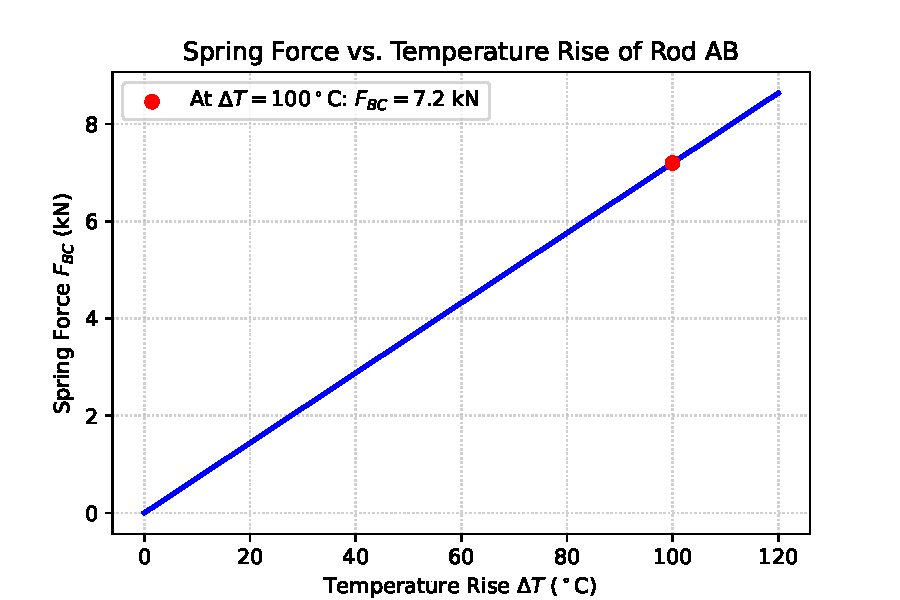
\includegraphics[width=0.85\columnwidth,keepaspectratio]{figs/q51.pdf}
\caption{Rod $AB$ connected in series with spring $BC$ under thermal loading}
\end{figure}
\begin{lstlisting}[frame=single, basicstyle=\rmfamily, escapeinside={(*@}{@*)}]
(*@\makebox[\dimexpr\linewidth-2\fboxsep-2\fboxrule\relax][c]{codes/ce1/q51.py}@*)
\end{lstlisting}
\begin{lstlisting}[frame=single, basicstyle=\rmfamily, escapeinside={(*@}{@*)}]
(*@\makebox[\dimexpr\linewidth-2\fboxsep-2\fboxrule\relax][c]{figs/q51.pdf}@*)
\end{lstlisting}

\end{enumerate}
